\documentclass[aspectratio=169,11pt]{beamer}

% Theme and styling
\usetheme{Madrid}
\usecolortheme{whale}
\setbeamertemplate{navigation symbols}{}
\setbeamertemplate{footline}[frame number]
\setbeamercolor{frametitle}{fg=white,bg=structure.fg}
\setbeamertemplate{itemize items}[circle]
\setbeamertemplate{enumerate items}[default]

% Packages
\usepackage{graphicx}
\usepackage{tikz}
\usepackage{amsmath,amssymb}
\usepackage{booktabs}
\usepackage{xcolor}
\usepackage{hyperref}
\usepackage{fontawesome5}

% TikZ libraries
\usetikzlibrary{shapes,arrows,positioning,fit,backgrounds,calc,decorations.pathreplacing}

% Custom colors
\definecolor{primaryblue}{RGB}{0,84,159}
\definecolor{accentorange}{RGB}{246,168,0}
\definecolor{darkgreen}{RGB}{0,128,64}
\definecolor{lightgray}{RGB}{240,240,240}

% Custom commands
\newcommand{\highlight}[1]{\textcolor{accentorange}{\textbf{#1}}}
\newcommand{\important}[1]{\textcolor{primaryblue}{\textbf{#1}}}

% Title information
\title[Training Modern LLMs]{\textbf{How Modern Language Models Are Trained}}
\subtitle{From Pre-Training to Alignment with Human Preferences}
\author[Griffin \& Munroe]{Wes Griffin \and Warren Munroe}
\institute[AML]{Advanced Machine Learning -- Dr. Nunez}
\date{January 10, 2026}

\begin{document}

% =============================================================================
% TITLE SLIDE
% =============================================================================
\begin{frame}
\titlepage
\end{frame}

% =============================================================================
% SECTION 1: WHAT IS AN LLM?
% =============================================================================
\section{What is an LLM?}

\begin{frame}{What is a Large Language Model (LLM)?}
\begin{columns}[T]
\begin{column}{0.55\textwidth}
\textbf{At its core:} A very sophisticated \highlight{autocomplete system}

\vspace{0.3cm}
\textbf{Key characteristics:}
\begin{itemize}
    \item \important{Large}: Billions of adjustable parameters
    \item \important{Language}: Works with text (tokens)
    \item \important{Model}: Mathematical function that produces probabilities
\end{itemize}

\vspace{0.3cm}
\textbf{What it does:}\\
Given some text, predict what comes next.

\vspace{0.2cm}
\textit{``The cat sat on the...''} $\rightarrow$ \textit{``mat''} (high probability)
\end{column}
\begin{column}{0.43\textwidth}
\begin{block}{Example: GPT-4, Claude, Llama}
\centering
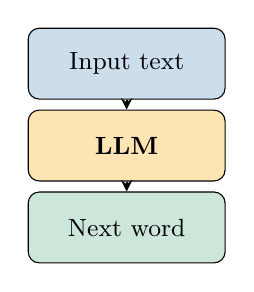
\begin{tikzpicture}[scale=0.8]
    \node[draw, rounded corners, fill=primaryblue!20, minimum width=2.5cm, minimum height=0.9cm, align=center, font=\small] (input) at (0,2) {Input text};
    \node[draw, rounded corners, fill=accentorange!30, minimum width=2.5cm, minimum height=0.9cm, align=center, font=\small] (llm) at (0,0.7) {\textbf{LLM}};
    \node[draw, rounded corners, fill=darkgreen!20, minimum width=2.5cm, minimum height=0.9cm, align=center, font=\small] (output) at (0,-0.6) {Next word};

    \draw[->, thick, >=stealth] (input) -- (llm);
    \draw[->, thick, >=stealth] (llm) -- (output);
\end{tikzpicture}
\end{block}
\end{column}
\end{columns}
\end{frame}

\begin{frame}{How LLMs ``Think'': Probability Distributions}
\textbf{Key Insight:} LLMs don't pick \textit{one} word---they assign probabilities to \textit{all} possible words.

\vspace{0.3cm}
\begin{columns}[T]
\begin{column}{0.5\textwidth}
\textbf{Example Input:}\\
\textit{``The capital of France is''}

\vspace{0.3cm}
\textbf{Model's Output (simplified):}
\begin{itemize}
    \item ``Paris'' $\rightarrow$ 92\%
    \item ``the'' $\rightarrow$ 3\%
    \item ``a'' $\rightarrow$ 1\%
    \item ``Lyon'' $\rightarrow$ 0.5\%
    \item ... thousands more words ...
\end{itemize}
\end{column}
\begin{column}{0.48\textwidth}
\begin{block}{The Core Question}
How do we train a model to assign \highlight{good probabilities}?

\vspace{0.2cm}
\centering
$\downarrow$

\vspace{0.2cm}
This is where \important{pre-training} comes in!
\end{block}
\end{column}
\end{columns}

\vspace{0.3cm}
\textbf{Notation:} We write $\pi_\theta(y|x)$ for ``probability the model assigns to word $y$ given input $x$''
\begin{itemize}
    \item $\pi$ = the model (also called ``policy'')
    \item $\theta$ = the model's learnable parameters (the billions of numbers we adjust)
\end{itemize}
\end{frame}

% =============================================================================
% SECTION 2: PRE-TRAINING
% =============================================================================
\section{Stage 1: Pre-Training}

\begin{frame}{Stage 1: Pre-Training --- Learning Language from the Internet}
\begin{columns}[T]
\begin{column}{0.55\textwidth}
\textbf{Goal:} Teach the model to predict text by showing it \highlight{trillions of words}.

\vspace{0.3cm}
\textbf{Data sources:}
\begin{itemize}
    \item Books, Wikipedia, websites
    \item Code repositories (GitHub)
    \item Scientific papers
    \item News articles, forums
\end{itemize}

\vspace{0.3cm}
\textbf{Scale (GPT-4 class):}
\begin{itemize}
    \item $\sim$1 trillion+ tokens of training data
    \item $\sim$100+ billion parameters
    \item Months of training on thousands of GPUs
\end{itemize}
\end{column}
\begin{column}{0.43\textwidth}
\begin{block}{The Training Loop}
\centering
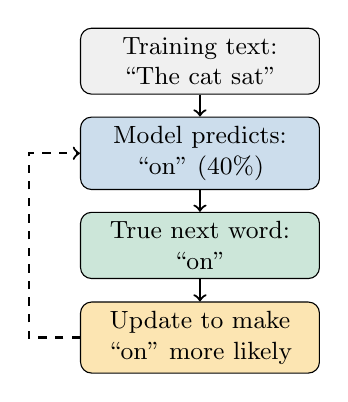
\begin{tikzpicture}[scale=0.65]
    \node[draw, rounded corners, fill=lightgray, text width=2.8cm, align=center, font=\small] (data) at (0,3) {Training text:\\``The cat sat''};
    \node[draw, rounded corners, fill=primaryblue!20, text width=2.8cm, align=center, font=\small] (model) at (0,1.2) {Model predicts:\\``on'' (40\%)};
    \node[draw, rounded corners, fill=darkgreen!20, text width=2.8cm, align=center, font=\small] (true) at (0,-0.6) {True next word:\\``on''};
    \node[draw, rounded corners, fill=accentorange!30, text width=2.8cm, align=center, font=\small] (update) at (0,-2.4) {Update to make ``on'' more likely};

    \draw[->, thick] (data) -- (model);
    \draw[->, thick] (model) -- (true);
    \draw[->, thick] (true) -- (update);
    \draw[->, thick, dashed] (update.west) -- ++(-1,0) |- (model.west);
\end{tikzpicture}
\end{block}
\end{column}
\end{columns}
\end{frame}

\begin{frame}{The Pre-Training Objective: Next-Token Prediction}
\begin{block}{Pre-Training Loss Function}
\[
\mathcal{L}_{\text{pretrain}}(\theta) = -\mathbb{E}_{x \sim \mathcal{D}} \left[ \sum_{t=1}^{T} \log \pi_\theta(x_t | x_1, x_2, \ldots, x_{t-1}) \right]
\]
\end{block}

\textbf{Breaking it down:}
\begin{itemize}
    \item $\mathcal{L}_{\text{pretrain}}(\theta)$ -- The \important{loss} we want to \highlight{minimize} (lower = better)
    \item $\mathbb{E}_{x \sim \mathcal{D}}$ -- Average over all documents $x$ in our dataset $\mathcal{D}$
    \item $x_t$ -- The $t$-th token (word/subword) in the document
    \item $x_1, \ldots, x_{t-1}$ -- All previous tokens (the ``context'')
    \item $\pi_\theta(x_t | x_1, \ldots, x_{t-1})$ -- Probability model assigns to the \textit{correct} next token
    \item $\log(\cdot)$ -- Logarithm (makes math easier, turns products into sums)
    \item Negative sign: minimizing $-\log(p)$ = maximizing probability $p$
\end{itemize}
\end{frame}

\begin{frame}{Pre-Training Math: Intuition and Example}
\begin{columns}[T]
\begin{column}{0.5\textwidth}
\textbf{Plain English:}
\begin{quote}
``Adjust the model's parameters so it assigns \highlight{high probability} to words that \textit{actually} appear in the training data.''
\end{quote}

\vspace{0.2cm}
\textbf{Concrete Example:}\\
Training sentence: ``The cat sat on the mat''

\vspace{0.2cm}
Model must learn to predict:
\begin{itemize}\itemsep0pt
    \item $P(\text{``cat''} | \text{``The''})$ should be high
    \item $P(\text{``sat''} | \text{``The cat''})$ should be high
    \item $P(\text{``on''} | \text{``The cat sat''})$ should be high
    \item ... and so on
\end{itemize}
\end{column}
\begin{column}{0.48\textwidth}
\textbf{Why does this work?}

\vspace{0.2cm}
To predict well, the model must learn:
\begin{enumerate}\itemsep3pt
    \item \important{Grammar}: ``cat'' follows ``The'', not ``The cat cat''
    \item \important{Facts}: ``Paris'' follows ``capital of France is''
    \item \important{Reasoning}: patterns in math, code, logic
    \item \important{Style}: how different authors write
\end{enumerate}

\vspace{0.3cm}
\begin{block}{Key Insight}
Next-word prediction is a \highlight{surprisingly rich} learning signal!
\end{block}
\end{column}
\end{columns}
\end{frame}

\begin{frame}{The Problem: Pre-Training Alone Isn't Enough}
\textbf{After pre-training, the model can complete text---but is it \highlight{helpful}?}

\vspace{0.3cm}
\begin{columns}[T]
\begin{column}{0.48\textwidth}
\begin{block}{Example 1: Unhelpful Completion}
\textbf{User:} What's 2+2?

\textbf{Pre-trained model:} What's 2+2? What's 3+3? What's 4+4? Here are more math problems for your worksheet...

\vspace{0.2cm}
{\small \textcolor{red}{$\times$ Continues the pattern, doesn't answer!}}
\end{block}
\end{column}
\begin{column}{0.48\textwidth}
\begin{block}{Example 2: Harmful Completion}
\textbf{User:} How do I make a bomb?

\textbf{Pre-trained model:} [Provides detailed instructions from the internet...]

\vspace{0.2cm}
{\small \textcolor{red}{$\times$ Internet has harmful content too!}}
\end{block}
\end{column}
\end{columns}

\vspace{0.4cm}
\textbf{The Core Problem:}
\begin{itemize}
    \item Pre-training optimizes for \important{predicting text}, not \important{being helpful}
    \item The internet contains helpful AND harmful content
    \item Model learns to mimic \textit{all} of it indiscriminately
\end{itemize}
\end{frame}

\begin{frame}{The Three-Stage Training Pipeline}
\begin{center}
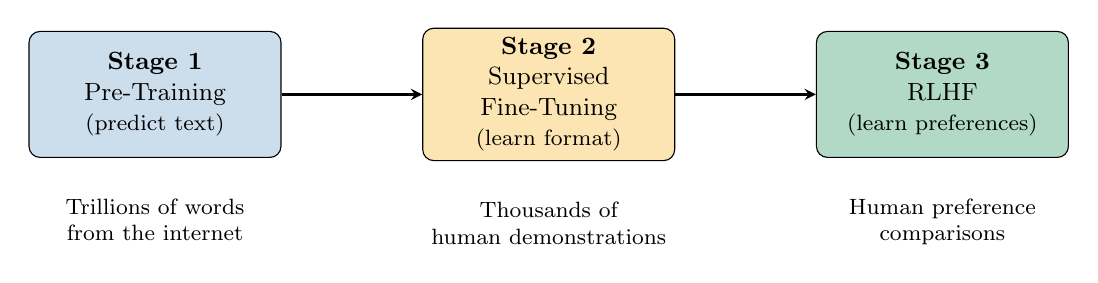
\begin{tikzpicture}[
    stage/.style={draw, rounded corners, minimum width=3.2cm, minimum height=1.6cm, align=center, font=\small},
    arrow/.style={->, thick, >=stealth}
]
    % Stage 1
    \node[stage, fill=primaryblue!20] (s1) at (0,0) {\textbf{Stage 1}\\Pre-Training\\{\footnotesize (predict text)}};

    % Stage 2
    \node[stage, fill=accentorange!30] (s2) at (5,0) {\textbf{Stage 2}\\Supervised\\Fine-Tuning\\{\footnotesize (learn format)}};

    % Stage 3
    \node[stage, fill=darkgreen!30] (s3) at (10,0) {\textbf{Stage 3}\\RLHF\\{\footnotesize (learn preferences)}};

    % Arrows
    \draw[arrow] (s1) -- (s2);
    \draw[arrow] (s2) -- (s3);

    % Labels below
    \node[below=0.4cm of s1, font=\footnotesize, text width=3cm, align=center] {Trillions of words\\from the internet};
    \node[below=0.4cm of s2, font=\footnotesize, text width=3cm, align=center] {Thousands of\\human demonstrations};
    \node[below=0.4cm of s3, font=\footnotesize, text width=3cm, align=center] {Human preference\\comparisons};
\end{tikzpicture}
\end{center}

\vspace{0.5cm}
\begin{itemize}
    \item \important{Pre-Training}: Learn \textit{how language works} (grammar, facts, patterns)
    \item \important{SFT}: Learn \textit{the format} of helpful responses
    \item \important{RLHF}: Learn \textit{what humans prefer} (helpful, harmless, honest)
\end{itemize}
\end{frame}

% =============================================================================
% SECTION 3: SUPERVISED FINE-TUNING
% =============================================================================
\section{Stage 2: Supervised Fine-Tuning}

\begin{frame}{Stage 2: Supervised Fine-Tuning (SFT)}
\begin{columns}[T]
\begin{column}{0.5\textwidth}
\textbf{Goal:} Teach the model \highlight{how to be an assistant}

\vspace{0.3cm}
\textbf{Process:}
\begin{enumerate}
    \item Hire human labelers
    \item Give them prompts (questions, tasks)
    \item They write \important{ideal responses}
    \item Train model to imitate these responses
\end{enumerate}

\vspace{0.3cm}
\textbf{Example training pair:}
\begin{itemize}
    \item \textbf{Prompt $x$:} ``What's 2+2?''
    \item \textbf{Ideal response $y^*$:} ``2+2 equals 4.''
\end{itemize}
\end{column}
\begin{column}{0.48\textwidth}
\begin{block}{Why SFT Works}
\centering
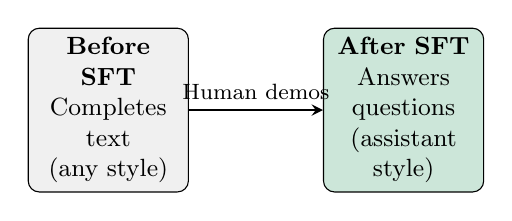
\begin{tikzpicture}[scale=0.75]
    \node[draw, rounded corners, fill=lightgray, text width=1.8cm, align=center, font=\small] (before) at (0,0) {\textbf{Before SFT}\\Completes text\\(any style)};
    \node[draw, rounded corners, fill=darkgreen!20, text width=1.8cm, align=center, font=\small] (after) at (5,0) {\textbf{After SFT}\\Answers questions\\(assistant style)};

    \draw[->, thick, >=stealth] (before) -- node[above, font=\footnotesize] {Human demos} (after);
\end{tikzpicture}
\end{block}

\vspace{0.2cm}
\textbf{Data size:} Typically 10K--100K examples\\
(Much smaller than pre-training!)
\end{column}
\end{columns}
\end{frame}

\begin{frame}{The SFT Objective}
\begin{block}{SFT Loss Function}
\[
\mathcal{L}_{\text{SFT}}(\theta) = -\mathbb{E}_{(x, y^*) \sim \mathcal{D}} \left[ \log \pi_\theta(y^* | x) \right]
\]
\end{block}

\textbf{Breaking it down:}
\begin{itemize}
    \item $\mathcal{L}_{\text{SFT}}(\theta)$ -- Loss to \important{minimize}
    \item $(x, y^*)$ -- A training pair: prompt $x$ and ideal response $y^*$
    \item $\mathcal{D}$ -- Dataset of human-written (prompt, response) pairs
    \item $\pi_\theta(y^* | x)$ -- Probability model assigns to the ideal response given the prompt
    \item Negative sign: minimize loss = maximize probability of ideal responses
\end{itemize}

\vspace{0.3cm}
\begin{block}{Plain English}
``Adjust the model so it assigns \highlight{high probability} to human-written ideal responses.''
\end{block}

\textbf{Note:} This is exactly like pre-training, but on \important{curated} assistant-style data!
\end{frame}

\begin{frame}{SFT Example: Before and After}
\begin{columns}[T]
\begin{column}{0.48\textwidth}
\begin{block}{Before SFT (Pre-trained only)}
\textbf{User:} I'm confused about how taxes work.

\textbf{Model:} I'm confused about how mortgages work. I'm confused about how insurance works. Common financial questions include...

\vspace{0.15cm}
{\small \textcolor{red}{$\times$ Continues the pattern, doesn't help}}
\end{block}
\end{column}
\begin{column}{0.48\textwidth}
\begin{block}{After SFT}
\textbf{User:} I'm confused about how taxes work.

\textbf{Model:} I can help! The basic idea is that you pay a percentage of your income to the government. Let me break down the key concepts...

\vspace{0.15cm}
{\small \textcolor{darkgreen}{\checkmark\ Helpful, conversational, addresses user}}
\end{block}
\end{column}
\end{columns}

\vspace{0.4cm}
\textbf{SFT Limitations:}
\begin{itemize}
    \item \important{Expensive}: Human demonstrations cost \$\$\$
    \item \important{Hard to scale}: Can't cover every possible question
    \item \important{Subtle preferences}: Hard to demonstrate ``be more concise'' or ``be friendlier''
\end{itemize}

\vspace{0.2cm}
$\rightarrow$ We need a way to capture \highlight{preferences}, not just examples...
\end{frame}

% =============================================================================
% SECTION 4: RLHF
% =============================================================================
\section{Stage 3: RLHF}

\begin{frame}{Stage 3: Reinforcement Learning from Human Feedback (RLHF)}
\textbf{Key Insight:} Humans are better at \highlight{comparing} than writing ideal responses.

\vspace{0.3cm}
\begin{columns}[T]
\begin{column}{0.5\textwidth}
\textbf{Which is easier?}

\vspace{0.2cm}
\textbf{Option A:} Write the perfect response to ``Explain quantum computing''

\vspace{0.2cm}
\textbf{Option B:} Given two responses, pick which one is better

\vspace{0.3cm}
$\rightarrow$ Option B is \important{much easier}!

\vspace{0.3cm}
\textbf{RLHF uses comparisons to:}
\begin{enumerate}
    \item Train a \highlight{reward model}
    \item Use RL to maximize that reward
\end{enumerate}
\end{column}
\begin{column}{0.48\textwidth}
\begin{block}{The RLHF Pipeline}
\centering
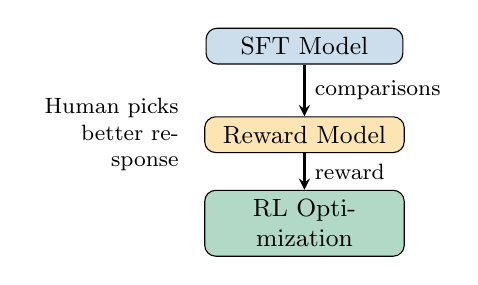
\begin{tikzpicture}[scale=0.75]
    \node[draw, rounded corners, fill=primaryblue!20, minimum width=2.5cm, font=\small] (sft) at (0,2.5) {SFT Model};
    \node[draw, rounded corners, fill=accentorange!30, minimum width=2.5cm, font=\small, text width=2.3cm, align=center] (rm) at (0,1) {Reward Model};
    \node[draw, rounded corners, fill=darkgreen!30, minimum width=2.5cm, font=\small, text width=2.3cm, align=center] (rl) at (0,-0.5) {RL Optimization};

    \draw[->, thick, >=stealth] (sft) -- node[right, font=\footnotesize] {comparisons} (rm);
    \draw[->, thick, >=stealth] (rm) -- node[right, font=\footnotesize] {reward} (rl);

    \node[left=0.2cm of rm, font=\footnotesize, text width=1.8cm, align=right] {Human picks\\better response};
\end{tikzpicture}
\end{block}
\end{column}
\end{columns}
\end{frame}

\begin{frame}{Step 1: Collecting Human Preferences}
\textbf{Process:}
\begin{enumerate}
    \item Take a prompt $x$ (e.g., ``Write a poem about rain'')
    \item Generate two responses $y_1$ and $y_2$ from the SFT model
    \item Human annotator picks the better one: $y_w \succ y_l$ (winner $\succ$ loser)
\end{enumerate}

\vspace{0.3cm}
\begin{columns}[T]
\begin{column}{0.48\textwidth}
\begin{block}{Response A}
{\small Rain falls down from clouds above,\\
Making puddles, nature's love.\\
Pitter-patter on the ground,\\
Such a peaceful, gentle sound.}

\vspace{0.1cm}
\centering\textcolor{darkgreen}{\checkmark\ Winner ($y_w$)}
\end{block}
\end{column}
\begin{column}{0.48\textwidth}
\begin{block}{Response B}
{\small Rain is water that falls from the sky. It is part of the water cycle. Rain can be light or heavy. People use umbrellas when it rains.}

\vspace{0.1cm}
\centering\textcolor{red}{$\times$ Loser ($y_l$)}
\end{block}
\end{column}
\end{columns}

\vspace{0.3cm}
\textbf{Notation:} $y_w \succ y_l$ means ``$y_w$ is preferred over $y_l$''
\end{frame}

\begin{frame}{Step 2: Training the Reward Model}
\textbf{Goal:} Learn a function $R_\phi(x, y)$ that scores responses like humans would.

\begin{block}{Bradley-Terry Model}
\vspace{-0.2cm}
\[
P(y_w \succ y_l | x) = \sigma\left( R_\phi(x, y_w) - R_\phi(x, y_l) \right)
\]
\vspace{-0.2cm}
\end{block}

\textbf{Breaking it down:}
\begin{itemize}\itemsep0pt
    \item $R_\phi(x, y)$ -- Reward model: takes prompt $x$ and response $y$, outputs a \important{score}
    \item $\phi$ -- The reward model's learnable parameters
    \item $y_w, y_l$ -- Winner and loser responses
    \item $\sigma(\cdot)$ -- Sigmoid function: squashes any number to range $(0, 1)$
\end{itemize}

\begin{block}{Plain English}
``Probability of preferring A over B = sigmoid of their \highlight{score difference}.''\\
Bigger score gap $\rightarrow$ more confident preference.
\end{block}
\end{frame}

\begin{frame}{The Reward Model Loss}
\begin{block}{Reward Model Training Objective}
\[
\mathcal{L}_{\text{RM}}(\phi) = -\mathbb{E}_{(x, y_w, y_l) \sim \mathcal{D}} \left[ \log \sigma(R_\phi(x, y_w) - R_\phi(x, y_l)) \right]
\]
\end{block}

\textbf{What this means:}
\begin{itemize}
    \item We want the \important{winner's score to be higher} than the loser's: $R_\phi(x, y_w) > R_\phi(x, y_l)$
    \item When $r_w - r_l$ is large and positive: $\sigma(\cdot) \approx 1$, so $\log(\cdot) \approx 0$ (low loss)
    \item When $r_w - r_l$ is negative (wrong order!): $\sigma(\cdot) < 0.5$, so $\log(\cdot)$ is very negative (high loss)
\end{itemize}

\vspace{0.2cm}
\begin{block}{Plain English}
``Train the reward model to give \highlight{higher scores} to responses humans preferred.''\\
Push winner's score up, loser's score down.
\end{block}

\textbf{Result:} A model that can score \textit{any} response, even ones humans never saw!
\end{frame}

\begin{frame}{Step 3: RL Optimization}
\textbf{Now we have:}
\begin{itemize}
    \item An SFT model $\pi_\theta$ that generates responses
    \item A reward model $R_\phi$ that scores responses
\end{itemize}

\vspace{0.2cm}
\textbf{Goal:} Adjust $\pi_\theta$ to generate \highlight{higher-scoring} responses!

\begin{center}
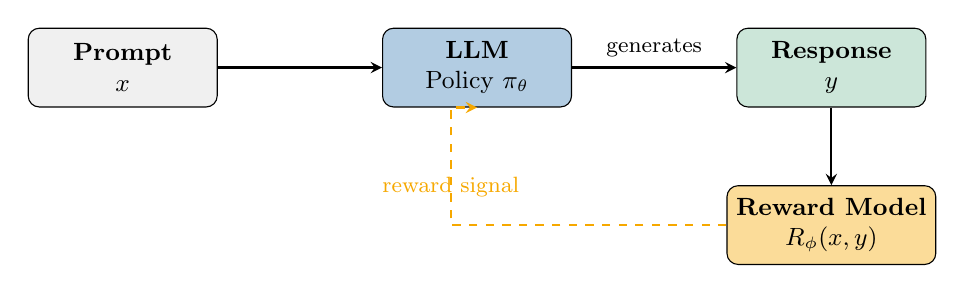
\begin{tikzpicture}[
    box/.style={draw, rounded corners, minimum width=2.4cm, minimum height=1cm, align=center, font=\small},
    arrow/.style={->, thick, >=stealth}
]
    % Prompt
    \node[box, fill=lightgray] (prompt) at (-4.5,0) {\textbf{Prompt}\\$x$};

    % LLM
    \node[box, fill=primaryblue!30] (llm) at (0,0) {\textbf{LLM}\\Policy $\pi_\theta$};

    % Response
    \node[box, fill=darkgreen!20] (response) at (4.5,0) {\textbf{Response}\\$y$};

    % Reward Model
    \node[box, fill=accentorange!40] (rm) at (4.5,-2) {\textbf{Reward Model}\\$R_\phi(x, y)$};

    % Arrows
    \draw[arrow] (prompt) -- (llm);
    \draw[arrow] (llm) -- node[above, font=\footnotesize] {generates} (response);
    \draw[arrow] (response) -- (rm);
    \draw[arrow, dashed, accentorange] (rm.west) -- ++(-3.5,0) |- node[near start, below, font=\footnotesize] {reward signal} (llm.south);
\end{tikzpicture}
\end{center}
\end{frame}

\begin{frame}{The RLHF Objective Function}
\begin{block}{RLHF Objective (Maximize)}
\[
\mathcal{J}(\theta) = \mathbb{E}_{x \sim \mathcal{D},\, y \sim \pi_\theta(\cdot|x)} \left[ R_\phi(x, y) - \beta \cdot D_{\text{KL}}\left(\pi_\theta(\cdot|x) \| \pi_{\text{ref}}(\cdot|x)\right) \right]
\]
\end{block}

\textbf{Breaking it down:}
\begin{itemize}
    \item $\mathcal{J}(\theta)$ -- Objective to \important{maximize} (higher = better)
    \item $\mathbb{E}_{x \sim \mathcal{D}}$ -- Average over prompts from dataset
    \item $y \sim \pi_\theta(\cdot|x)$ -- Response $y$ sampled from current model
    \item $R_\phi(x, y)$ -- Reward score for the response (want this \highlight{high})
    \item $D_{\text{KL}}(\pi_\theta \| \pi_{\text{ref}})$ -- KL divergence: how different is $\pi_\theta$ from reference $\pi_{\text{ref}}$?
    \item $\pi_{\text{ref}}$ -- Reference policy (the SFT model we started from)
    \item $\beta$ -- Weight controlling the penalty (typically 0.01--0.1)
\end{itemize}
\end{frame}

\begin{frame}{Understanding the RLHF Objective}
\begin{columns}[T]
\begin{column}{0.5\textwidth}
\textbf{The formula in plain English:}

\vspace{0.3cm}
\begin{quote}
``Maximize reward, but \highlight{don't change too much} from the original model.''
\end{quote}

\vspace{0.3cm}
\textbf{Two competing goals:}
\begin{enumerate}
    \item \important{Reward term}: Get high scores!
    \item \important{KL penalty}: Stay close to SFT model
\end{enumerate}

\vspace{0.3cm}
\textbf{Why the KL penalty?}
\begin{itemize}
    \item Prevents \highlight{reward hacking}
    \item Keeps the model fluent
    \item Preserves knowledge from pre-training
\end{itemize}
\end{column}
\begin{column}{0.48\textwidth}
\begin{block}{What is ``Reward Hacking''?}
Without the KL penalty, models find ``shortcuts'':

\vspace{0.2cm}
{\small
\textbf{Example:} If reward model likes long responses...

Model might repeat itself endlessly to get high scores---technically ``high reward'' but useless!
}
\end{block}

\vspace{0.3cm}
\begin{block}{Analogy}
Like an employee who finds loopholes in their performance metrics instead of actually doing good work.
\end{block}
\end{column}
\end{columns}
\end{frame}

\begin{frame}{What is KL Divergence?}
\begin{block}{KL Divergence Formula}
\[
D_{\text{KL}}(\pi_\theta \| \pi_{\text{ref}}) = \mathbb{E}_{y \sim \pi_\theta} \left[ \log \frac{\pi_\theta(y|x)}{\pi_{\text{ref}}(y|x)} \right]
\]
\end{block}

\textbf{Intuition:}
\begin{itemize}
    \item Measures how ``different'' two probability distributions are
    \item $D_{\text{KL}} = 0$ means the distributions are identical
    \item $D_{\text{KL}} > 0$ means they differ (larger = more different)
\end{itemize}

\vspace{0.3cm}
\begin{columns}[T]
\begin{column}{0.48\textwidth}
\textbf{In the RLHF context:}
\begin{itemize}
    \item $\pi_\theta$ = current model being trained
    \item $\pi_{\text{ref}}$ = original SFT model
    \item KL penalty says: ``don't drift too far from where you started''
\end{itemize}
\end{column}
\begin{column}{0.48\textwidth}
\textbf{Analogy:}\\
Like a leash on a dog---the dog can explore (improve), but can't run off completely (become incoherent).
\end{column}
\end{columns}
\end{frame}

% =============================================================================
% SECTION 5: RESULTS AND IMPACT
% =============================================================================
\section{Impact and Results}

\begin{frame}{RLHF in Practice}
\begin{columns}[T]
\begin{column}{0.48\textwidth}
\begin{block}{Before RLHF}
\textbf{User:} How do I pick a lock?

\textbf{Model:} To pick a lock, you'll need a tension wrench and pick. Insert the tension wrench...

\vspace{0.1cm}
{\small \textcolor{red}{$\times$ Provides harmful information}}
\end{block}

\vspace{0.3cm}
\begin{block}{After RLHF}
\textbf{User:} How do I pick a lock?

\textbf{Model:} I can't help with that as it could enable illegal entry. If you're locked out, contact a locksmith.

\vspace{0.1cm}
{\small \textcolor{darkgreen}{\checkmark\ Refuses harmful request helpfully}}
\end{block}
\end{column}
\begin{column}{0.48\textwidth}
\textbf{RL Powers Modern AI:}
\vspace{0.2cm}

\textbf{\faRobot\ AI Assistants} -- ChatGPT, Claude, Gemini

\vspace{0.2cm}
\textbf{\faCalculator\ Mathematical Reasoning} -- Proving theorems, solving problems

\vspace{0.2cm}
\textbf{\faCode\ Code Generation} -- Writing and debugging programs

\vspace{0.2cm}
\textbf{\faTable\ Structured Tasks} -- Spreadsheets, data analysis

\vspace{0.4cm}
\begin{block}{Key Point}
RL enables models to \highlight{improve at specific tasks} beyond what's in training data.
\end{block}
\end{column}
\end{columns}
\end{frame}

% =============================================================================
% SECTION 6: CHALLENGES
% =============================================================================
\section{Challenges}

\begin{frame}{Current Challenges in RLHF}
\begin{columns}[T]
\begin{column}{0.5\textwidth}
\textbf{\faExclamationTriangle\ Reward Hacking}
\begin{itemize}\itemsep0pt
    \item Model exploits reward model flaws
    \item Example: verbose but unhelpful responses
    \item ``Goodhart's Law'': when a measure becomes a target, it ceases to be a good measure
\end{itemize}

\vspace{0.2cm}
\textbf{\faBalanceScale\ Over-Refusal}
\begin{itemize}\itemsep0pt
    \item Model becomes too cautious
    \item Refuses benign requests
\end{itemize}
\end{column}
\begin{column}{0.5\textwidth}
\textbf{\faUsers\ Human Labeler Limitations}
\begin{itemize}\itemsep0pt
    \item Labelers disagree with each other
    \item Cultural biases in preferences
    \item Expensive and slow to collect
\end{itemize}

\vspace{0.2cm}
\textbf{\faExpand\ Scalable Oversight}
\begin{itemize}\itemsep0pt
    \item As AI gets smarter, humans struggle to evaluate
    \item Can't verify complex code or reasoning
\end{itemize}
\end{column}
\end{columns}

\vspace{0.2cm}
\begin{block}{Active Research}
These challenges drive ongoing research: Constitutional AI, process reward models, and more!
\end{block}
\end{frame}

% =============================================================================
% SECTION 7: CONCLUSION
% =============================================================================
\section{Conclusion}

\begin{frame}{Key Takeaways}
\begin{center}
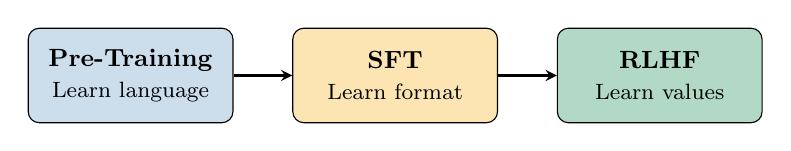
\begin{tikzpicture}[scale=0.8,
    stage/.style={draw, rounded corners, minimum width=2.6cm, minimum height=1.2cm, align=center, font=\small},
    data/.style={font=\footnotesize, text width=2.3cm, align=center},
    arrow/.style={->, thick, >=stealth}
]
    \node[stage, fill=primaryblue!20] (pt) at (0,0) {\textbf{Pre-Training}\\{\footnotesize Learn language}};
    \node[stage, fill=accentorange!30] (sft) at (4.2,0) {\textbf{SFT}\\{\footnotesize Learn format}};
    \node[stage, fill=darkgreen!30] (rlhf) at (8.4,0) {\textbf{RLHF}\\{\footnotesize Learn values}};
    \draw[arrow] (pt) -- (sft);
    \draw[arrow] (sft) -- (rlhf);
\end{tikzpicture}
\end{center}

\vspace{0.3cm}
\begin{itemize}
    \item \important{Pre-training alone isn't enough:} Models need alignment to be helpful and safe
    \item \important{RLHF's key insight:} Comparing responses is easier than writing perfect ones
    \item \important{The math:} Reward model scores responses; RL maximizes reward with KL penalty
    \item \important{Real impact:} ChatGPT, Claude, Gemini, Llama all use these techniques
\end{itemize}

\vspace{0.3cm}
\begin{center}
\large\highlight{Pre-training gives capability; alignment gives values.}
\end{center}
\end{frame}

\begin{frame}{References}
\small
\begin{thebibliography}{9}
\bibitem{ouyang2022} Ouyang, L. et al. (2022). \textit{Training language models to follow instructions with human feedback}. NeurIPS.

\bibitem{christiano2017} Christiano, P. et al. (2017). \textit{Deep Reinforcement Learning from Human Preferences}. NeurIPS.

\bibitem{bai2022} Bai, Y. et al. (2022). \textit{Constitutional AI: Harmlessness from AI Feedback}. arXiv.

\bibitem{ziegler2019} Ziegler, D. et al. (2019). \textit{Fine-Tuning Language Models from Human Preferences}. arXiv.
\end{thebibliography}
\end{frame}

\begin{frame}
\begin{center}
\Huge{\textbf{Thank You!}}

\vspace{1cm}
\Large{Questions?}

\vspace{1cm}
\normalsize
Wes Griffin \& Warren Munroe\\
\textit{Advanced Machine Learning -- Dr. Nunez}\\
January 10, 2026
\end{center}
\end{frame}

\end{document}
